\chapter{Metodologia}
\label{chap:meto}
\begin{flushright}
	"Nada é permanente, exceto a mudança." \\
	\ \\
	(Heráclito)
\end{flushright}

O fluxo metodológico utilizado pelo projeto seguiu uma idealização do Desenvolvimento de Produtos, onde é constituído por três principais etapas: Projeto Conceitual, Projeto Detalhado e Confecção, conforme demonstrado na figura~\ref{fig:metod}.  

\begin{figure}[h!]										\caption{Representação do Fluxo Metodológico}
	\label{fig:metod}		
	\centering										
	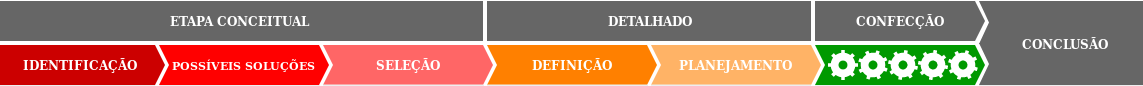
\includegraphics[width=1\textwidth]{metod.png}
	\source{Autores, 2019}		
\end{figure}

\section{Etapa Conceitual}
A etapa conceitual, foi caracterizada pela realização de outras três subetapas: Identificação, Levantamento de Possíveis Soluções e Seleção.

A etapa de identificação foi caracterizada pela definição dos requisitos do cliente e dos requisitos técnicos do projeto que serviram como guia para caracterizar a busca da solução.

A etapa seguinte, Levantamento de Possíveis Soluções, abrigou um SOTA, do inglês \textit{State of the Art}, que se trata de um estudo do estado da arte ou um \textit{Benchmarking} das principais soluções existentes no mercado, tanto nacional quanto internacional.

A etapa de Seleção foi o momento de se realizar a finalização do conceito, trazendo uma definição para o que viria a ser o design do protótipo, tal como a seleção inicial de componentes do sistema mecatrônico, e ainda a forma de apresentação dos conteúdos teóricos abordados.

Ainda na etapa de Seleção, foi realizado também um estudo das principais metodologias de ensino condizentes com o ensino da robótica e com o propósito deste projeto.

\section{Projeto Detalhado} 
A segunda etapa, o Projeto Detalhado, foi caracterizado por duas subetapas, que foram: Definição e Planejamento.

A etapa de Definição foi responsável pela especificação funcional dos elementos do projeto, da finalização do design do protótipo, da especificação dos conteúdos que seriam abordados na parte teórica, e pela definição da forma como esses conteúdos seriam passados para os estudantes, tanto na sua porção teórica, quanto na sua porção prática e intercomunicação entre ambas. Houve ainda a definição do método de fabricação das peças do protótipo físico.

Dando continuidade veio a etapa de Planejamento que foi responsável pela elaboração de toda a ordem a ser empregada na confecção dos materiais. Nesta etapa foram elaboradas a arquitetura mecatrônica do projeto, a separação dos componentes, o planejamento de fabricação das peças do protótipo físico e a definição do local onde os materiais teóricos seriam disponibilizados, tal como sua ordem de visualização e a organização disso de uma forma amigável para o estudante.

\section{Etapa de Confecção}
A última etapa foi a etapa de confecção, onde de fato todos os materiais teóricos foram elaborados e disponibilizados, o protótipo físico foi fabricado, montado e testado. Houve ainda a confecção dos pacotes de software utilizados, a instalação e configuração dos hardwares e seus testes.


